\documentclass[8pt]{article}
\usepackage{multicol}
\usepackage{amssymb,amsmath,latexsym}
\usepackage{graphicx}
\usepackage{caption}
\usepackage[utf8]{inputenc}
\newenvironment{hangingpar}[1]
{\begin{list}
		{}
		{\setlength{\itemindent}{-#1}%%'
			\setlength{\leftmargin}{#1}%%'
			\setlength{\itemsep}{0pt}%%'
			\setlength{\parsep}{\parskip}%%'
			\setlength{\topsep}{\parskip}%%'
		}
		\setlength{\parindent}{-#1}%%
		\item[]
	}
	{\end{list}}

\setlength{\oddsidemargin}{-0.25in} % Left margin of 1 in + 0 in = 1 in
\setlength{\textwidth}{7in}   % Right margin of 8.5 in - 1 in - 6.5 in = 1 in
\setlength{\topmargin}{-.75in}  % Top margin of 2 in -0.75 in = 1 in
\setlength{\textheight}{9in}  % Lower margin of 11 in - 9 in - 1 in = 1 in

\renewcommand{\baselinestretch}{1.5} % 1.5 denotes double spacing. Changing it will change the spacing

\begin{document}
\title{Automatic Prediction of Substance Abuse Using Supervised Learning}
\author{Matías Grinberg}
\date{\today}
\maketitle
\abstract{In this paper a proof-of-concept reduced questionnaire is developed using a machine learning classifier algorithm, so that its response data would then be given as input to predict a probability of potential drug abuse, screening subjects in risk. The data used for training the algorithm came from two national-wide census, and proved to be sufficient for a decent performing classifier (avg. ROC AUC = 0.90). This results further demonstrate that the use of machine learning for the development of innovative diagnostic tools is potentially a very fruitful research line.

\begin{multicols}{2}

\section{Introduction}
Substance related disorders are among the most common and harmful of the mental disorders (First, 2013). This individual phenomenon has important repercussions in every level of society, hindering it profoundly starting with the intra-personal dimension and scaling to affect the economy and homeland security of a country via the illicit  traffic of certain compounds. It is the product of uncountable etiologically significant factors of diverse nature, encompassing psychological, social, genetic and cultural realms. The presence of a substance abuse disorder is likely to disrupt most areas of an individual's life, from health habits to social relationships, and there is robust evidence that it is often associated with reduced life expectancy, depending on the used substance and the pattern of use. Certain patterns of abuse are also correlated with the diminished frequency of immunogenic activities, defined by patterns of actions directed to protect and improve general health (Morrison \& Bennett, 2008), like physical exercise, further harming life quality and longevity. Given that a healthy state of being, as defined by the World Health Organization, requires not only the absence of sickness, but optimal wellbeing in physical, mental and social spheres, substance abuse is a top priority issue to address. 

In the fifth edition of the Diagnostic and Statistical Manual of Mental Disorders (DSM-5), a widely used psychiatric reference, the term "substance-related disorder" refer to psychiatric conditions associated with drugs of abuse, the side effects of medication, and toxin-induced states. There are two types of substance-related diagnoses in DSM-5: the Substance Use Disorders, which describe a pattern of problematic substance use, and the Substance-Induced Disorders, that includes Substance Intoxication, Substance Withdrawal, and Substance/Medication-Induced
Mental Disorders), which describe direct behavioral correlates of the effect of substances on the central nervous system. In this paper, the machine learning algorithm classifies an individual as prone to substance use disorder for each of the selected substances (alcohol, cannabis, tobacco), roughly using the DSM criteria to construct the classification categories and maintain certain external reliability. Nonetheless, it is regarded that the strict adherence to this criteria is not as important as the model performance, so that while it may not perfectly coincide with the DSM, the accurate prediction of an ad hoc, well defined drug abuse construct has notable value for scalable automatic psychiatric diagnosis. 

Machine learning (ML) is a growing field in computer science and mathematical statistics, and a state-of-the-art technology that is facilitating notable advances in numerous and diverse areas. In the field of neuroscience, it has been successfully used in applications such as neuroimaging analysis (Tagliazzuchi et al, 2012), psychiatric diagnosis (Bedi et al 2015), and facial gestural analysis (Barlett, 2014). In relationship to this new technological toolkit, a new area of mental health has sprouted: computational psychiatry, to which this work may belong. This paper provides innovative research in the use of ML to develop a screening questionnaire to classify subjects at risk of drug abuse, facilitating primary prevention. 

This prevention of substance related disorders contemplates the high dimensionality of the determinants that ultimately result in the disorder from a broader view than the traditional individual-restrictive approach (Saforcada, 1999). This determinants are taken into account in the feature selection part of the process, serving as hypotheses regarding which of the variables will show predictive capability. The antecedents that relate to drug consumption can be categorized into distal and proximal determinants. In the first group, we locate peer and social groups that influence the tendency to consume, and in the illicit cases, the availability of access. Family interactions, and previous parental drug use are also possible predictors. In the individual scope of distal determinants, we find early learning, previous drug experiences and genetic inheritance (Sadock \& Sadock, 2011). The education received about drug consumptions is an important factor to take into account. . In the immediate group of determinants, we find, non exhaustively, the licensing laws that regulate drug use, social peer pressure, substance availability, related cultural constructs, demographic variables. On an individual level, some personality traits, e.g. sensation seeking (Jones et al, 2016), have a considerable influence on drug use, as does mood states, cognitive appraisal tendencies, and coping strategies. It is expected that the level of occupation of the individual will be correlated with the amount of drug consumption, given a possible feedback loop between free time, drug use and suboptimal productivity. The educational background, sociodemographic status, and cognitive perception of drug use, are also expected to be influential. The age of first consumption is also of particular interest, as it indicates access to the substance, possibly a tendency in the social context to consume, and it could possibly predispose to future drug disorders (Nielsen, 2012). Another specially interesting variable to account for, is the perceived risk of drug consumption, which will most likely influence its future use. This cognitive construct could be easily targeted by health promoting campaigns, so verifying its importance could prove useful.

\section{Data}
For this work the 2008 and 2011 census data of the \textit{Encuesta Nacional sobre Prevalencias de Consumo de Sustancias Psicoactivas} (ENPreCoSP) was used, which is carried out by the National Institute of Statistics and Census (INDEC) and the Ministry of Health of Argentina with the objective of determining the prevalence and incidence of psychoactive drug consumption in general population, and gain insight about the socio-economic, contextual and personal determinants. The total data comprises 68546 individual observations, consisting of 272 
variables (mainly multiple-choice question responses) that aim to reflect socio-economic status, and the characteristics of drug use. The sampling was carried out in a probabilistic stratified fashion, with 4 levels of increasing specificity: \textit{departamento, área, vivienda} and \textit{individuo}. For this last stratus, a Kish table was used for probabilistic selection. The data was recollected by personnel of the \textit{Direcciones Provinciales de Estadística} respective to each Argentinean province, trained specifically for the census. This collective applied the questionnaire, available in the link provided in the bibliography, in second person.
 
\begin{center}
	\captionof{figure}{Categorical index of variables}
	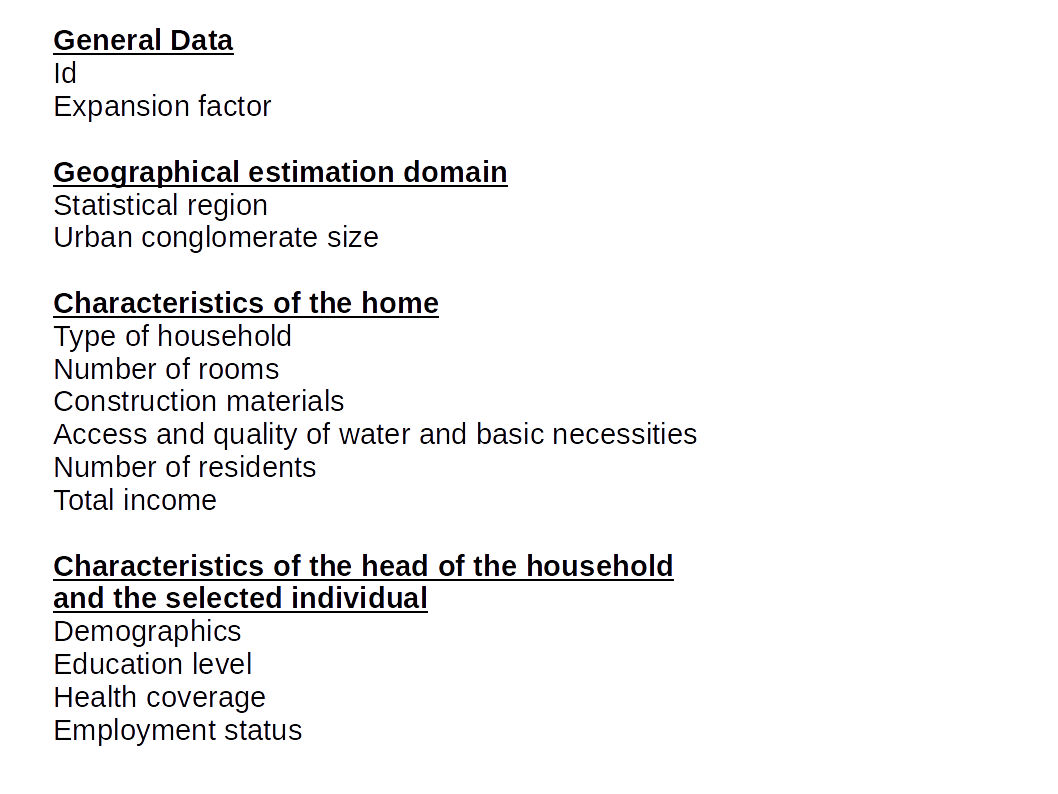
\includegraphics[width=.4\textwidth]{vars1.png}
	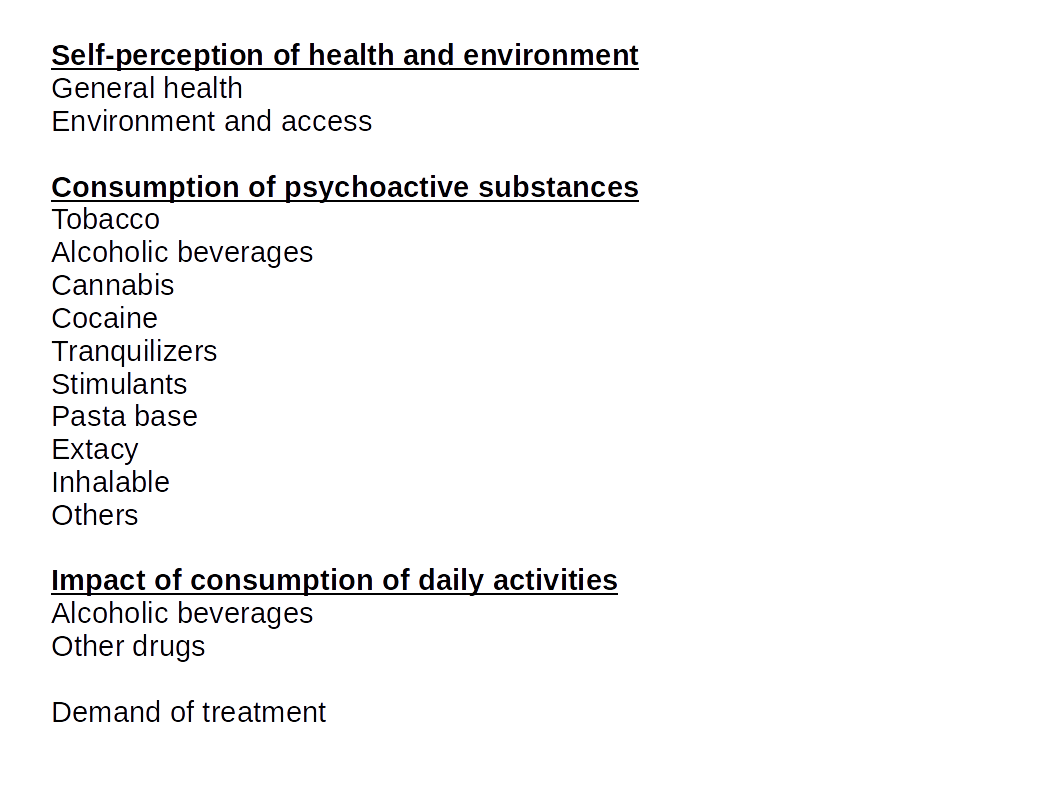
\includegraphics[width=.4\textwidth]{vars2.png}
\end{center}

The target variable was constructed taking in consideration the DSM-5 criteria for drug abuse, although this was not strict. A ground criteria, as hinted by the bibliography, was unhealthy habits, meaning that for example a small amount of periodic cigarette consumption was enough to qualify as a target. It is considered that the criteria used for classification is not as important as the actual predictive capability, so that as long as the target is well-defined and accurately classified, the algorithm serves a valuable use. Regarding cannabis, the target was defined by the past or current presence one or more of: almost daily consumption; overwhelming desire to consume; manifestation of tolerance buildup; impact on behavior; being unable to control consumption; or impact on health. For alcohol: the consumption of 20 or more drinks a week; drinking approximately 2 of 3 days; having had a work related problem related to alcohol consumption; having been drunk 3 or more times in the last 30 days; having suspended more than 9 days of activity in the last 12 months as a consequence of consumption. For tobacco consumption, which had a poorer sub-questionnaire, the criteria was more than 10 cigarettes per month, or a daily average superior to 0. The exact formulation of the construction heuristic is available with the rest of the code. 
\begin{center}
	\captionsetup[figure]{labelformat=empty, font=small}
	\captionof{figure}{DSM-5 Criteria and available data (e.g cannabis)}
	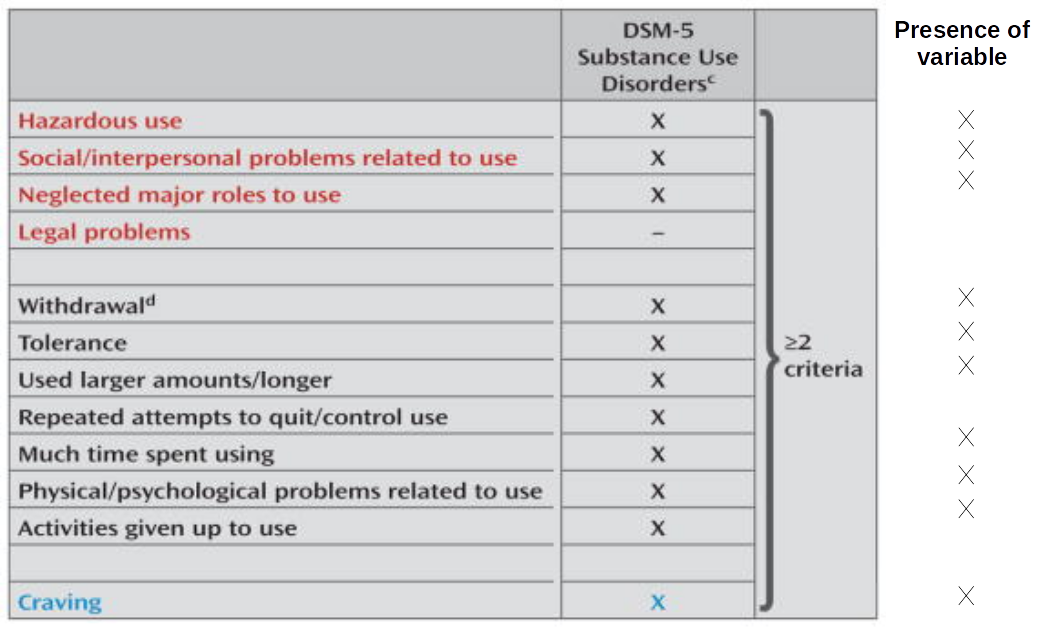
\includegraphics[width=.55\textwidth]{dsm.png}
	\captionsetup[figure]{labelformat=empty, font=small}
	\captionof{figure}{*Partially retrieved from Hasin et al 2013}
\end{center}

\section{EDA and Preprocessing}

An exploratory data analysis was carried out to attest for missing values and outliers. The distribution of multiple variables was studied to asses robustness. Regarding data imputation, a modelling strategy was used for the machine learning algorithms different from decision trees or ensambles like Random Forests or the best performant boosting tree, XGBoost, both which natively supports null values. Linear regression models where fitted for each dataset, and for each feature the linear regression was fitted with the remaining variables, resulting in the output used to fill null values. Nonetheless, this was only relevant previous to the use of XGBoost. Outliers where removed by truncation at the 0.0001 and 0.9999 quantiles. Correlation between all variables was measured with Spearman correlation coefficient, to contemplate colinearity that could interfere with the modelling. Also, variance thresholding was used to discard uninformative variables. The variables were mostly ordinal, so a one-hot-encoding (or dummie encoding) scheme was used, splitting each posible variable response into a separate column, and generating a (0,1) sparse matrix.

The distribution of cannabis and cocaine drug abuse cases was heavily skewed, with a relative frequency of less than 1\%. To correct this imbalance during fitting, two approaches were used. First, bootstrapping sampling of the data was carried out using Synthetic Minority Over-sampling Technique (SMOTE). Secondly, the hyperparameters of the boosting model and the metric score used, prioritized the recall of the lesser positive cases.

All the code for this work was produced using the Jupyter Notebook framework using the Python language, mainly with the Pandas and Sci-Kit Learn packages, for data processing, and for machine learning respectively. The code for this procedure is accessible in GitHub (see References). The LaTeX code containing this paper will also be available in the same repository.


\section{Modelling}
The machine learning algorithm used for supervised learning was XGBoost. In machine learning the objective is, given a matrix $x$ of input vectors, or predictor variables, and a paired vector $y$, the target, to approximate a function $\Hat{F}(x)$ that minimizes the expected value of a defined loss function $L(y, F(x))$ over the joint probability distribution $p(y, x)$ (Friedman, 2001).
\begin{equation*}
\Hat{F}(x) = argmin E_{x, y}L(y, \Hat{F}(x))
\end{equation*}
 
The used Extreme Gradient Boosting (XGBoost) algorithm approximates $\Hat{F}$ function using a boosting ensamble of decision trees. Unlike Random Forests, which is an ensemble of randomly generated decision trees, XGBoost fits each successive tree using the residual errors of the previous one, thus improving, or "boosting" the algorithm. Further algorithmic and mathematical details of the implementation are beyond the scope of this paper (for more information see Chen, 2016).

To avoid overfitting the estimated function to the available data, and too high variance that would make the model unable to generalize, the loss function was adjusted using 5-fold cross validation. This consists of alternatively choosing a fifth of the dataset as a test set, and using the remaining $4/5$ part as training. The model hyperparameters $H$ were set by a randomized search of parameter space, so to maximize the mean of the resulting loss function corresponding to each of the five instances of cross validation. The selected loss function for classification was the recall score $\frac{TP}{TP + FN}$, where T = True, F = False, P = Positive and N = Negative. 

\begin{equation*}
H = argmax(\frac{1}{n}\sum_{cv = 1}^{5}\frac{TP}{TP + FN})
\end{equation*}

Once the algorithm was fitted, a manual forward recursive feature elimination was carried out, selecting the features that proved most important for the trained model. Using this methodology, a dimensionality reduction of 86\% was accomplished, while maintaining similar performance scores. For model comparison, the area under the Receiver Operating Characteristic curve, which corresponds to the plot of True Positive Rate on the $y$ axis False Positive Rate on the $x$ axis, was computed.  

\section{Conclusion}

The hypothesis regarding potential determinant variables were mostly supported by the results. As it was expected, some of the predictive capacity of the algorithm emerged from: age of first consumption; employment condition; educational background; percieved risk of drug use; ease of access; characteristics of the home and reported curiosity to consume. This supports the psycho-bio-social approach to mental health, reflecting that the presence of the disorder depends on the confluence of diverse factors such as the cognitive beliefs about substance use or the social interaction with peers and family, also sociodemographic factors as age, education, sociocultural context or the household conformation and commodities. This drives the idea of implementing wide-reaching primary care campaigns to diminish drug use, by targeting specific beliefs and social affects.
The mean AUC ROC score for all models was ~0.9, being 0.5 the baseline of null information gain. This conveys sufficient evidence that this models could provide a solid tools for early diagnosis, serving for primary prevention and so improving general wellbeing efficiently. We see in the classification reports that precision of all models, for both positive and negative cases are extremely high, while the recall, or sensitivity scores are considerably weaker. This can be directly balanced by thresholding, or modifying the default 0.5 value by which the classifier discriminates positives and negative cases. 
The models maintain good performance, even using only the 38 most important variables as input. This resulting predictors correspond to the items that are to be used in the screening questionnaire, which would in turn yield results with the displayed reliability. 

\begin{center}
	\captionof{figure}{Classification report of 3 classifiers.}
	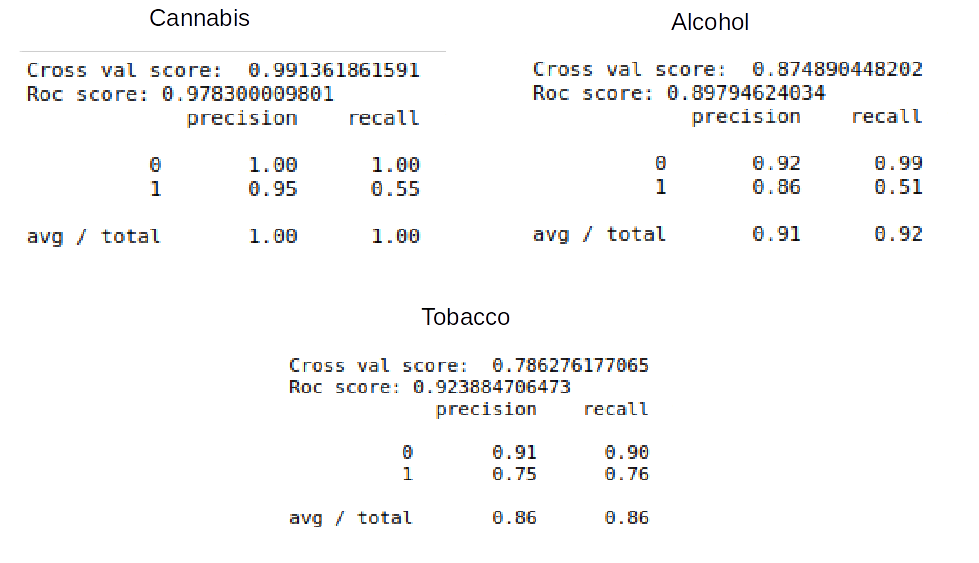
\includegraphics[width=.4\textwidth]{classif.png}
	\captionsetup[figure]{labelformat=empty, font=small}
\end{center}

This evidence suggests that a process similar to the one described here might be considerably useful in diagnosis of disorders related to substance abuse. Further tuning of the model parameters, as well as exploring other types of ML processing, are viable ways to improve model performance. More importantly, the potential use of this tools for refinement of the original census questionnaire, in conjunction with ML algorithms, suggests promising potential results.

\end{multicols}

\begin{thebibliography}{0}
\end{thebibliography}

\begin{hangingpar}{2em}

American Psychiatric Association. (2013). Diagnostic and statistical manual of mental disorders (5th ed.). Washington, DC: Author.

Bartlett, M. S., Littlewort, G., Lainscsek, C., Fasel, I., \& Movellan, J. (2004, October). Machine learning methods for fully automatic recognition of facial expressions and facial actions. In Systems, Man and Cybernetics, 2004 IEEE International Conference on (Vol. 1, pp. 592-597). IEEE.
ISO 690	

Bedi, G., Carrillo, F., Cecchi, G. A., Slezak, D. F., Sigman, M., Mota, N. B. \& Corcoran, C. M. (2015). Automated analysis of free speech predicts psychosis onset in high-risk youths. npj Schizophrenia, 1, 15030.

Chen, T., \& Guestrin, C. (2016, August). Xgboost: A scalable tree boosting system. In Proceedings of the 22nd acm sigkdd international conference on knowledge discovery and data mining (pp. 785-794). ACM.

ENPreCoSP questionnaire example and documentation available in http://www.indec.gob.ar/bases-de-datos.asp

First, M. B. (2013). DSM-5 handbook of differential diagnosis. American Psychiatric Pub.

Friedman, J. H. (2001). Greedy function approximation: a gradient boosting machine. Annals of statistics, 1189-1232.

Jones, T. M., Hill, K. G., Epstein, M., Lee, J. O., Hawkins, J. D., \& Catalano, R. F. (2016). Understanding the interplay of individual and social–developmental factors in the progression of substance use and mental health from childhood to adulthood. Development and psychopathology, 28(3), 721-741.

Hasin, D. S., O’Brien, C. P., Auriacombe, M., Borges, G., Bucholz, K., Budney, A., \& Schuckit, M. (2013). DSM-5 criteria for substance use disorders: recommendations and rationale. American Journal of Psychiatry, 170(8), 834-851.

Sadock, B. J., \& Sadock, V. A. (2011). Kaplan and Sadock's synopsis of psychiatry: Behavioral sciences/clinical psychiatry. Lippincott Williams \& Wilkins.

Morrison, V., Bennett, P., Parga, M. X. F., Franco, V. R., Elvira, A. C., \& Fidalgo, M. M. (2008). Psicología de la salud. Pearson.

Nielsen, D. A., Utrankar, A., Reyes, J. A., Simons, D. D., \& Kosten, T. R. (2012). Epigenetics of drug abuse: predisposition or response. Pharmacogenomics, 13(10), 1149–1160. http://doi.org/10.2217/pgs.12.94

Saforcada, E. (1999). Análisis de las concepciones y prácticas en salud. Psicología Sanitaria. Análisis crítico de los sistemas de atención de la salud, 69-104.

Tagliazucchi, E., von Wegner, F., Morzelewski, A., Borisov, S., Jahnke, K., \& Laufs, H. (2012). Automatic sleep staging using fMRI functional connectivity data. Neuroimage, 63(1), 63-72.

All code available in https://github.com/Cerebrock/AutomaticPredictionDrugAbuse

\end{hangingpar}
\end{document}